\documentclass[9pt]{beamer}
\usetheme{Boadilla}
\usepackage{tikz}
 \usepackage[english]{babel}
 \usepackage{amsmath}
 \usepackage{amsfonts}
 \usepackage{amssymb}
 \usepackage{amsthm}
 \usepackage{array}
 \newcommand{\tabitem}{%
  \usebeamertemplate{itemize item}\hspace*{\labelsep}}
 \usepackage{mathtools}
 \DeclarePairedDelimiterX{\inp}[2]{\langle}{\rangle}{#1, #2}
 \usepackage[utf8]{inputenc}
 \usepackage{dsfont}
 \usetikzlibrary{patterns}
 \usepackage{graphicx}
 \graphicspath{{"../Output/"}}
 \usepackage[export]{adjustbox}
 \usepackage{mathrsfs}
 \usepackage{bbold}
\usetikzlibrary{mindmap,trees,shadows}
\usepackage{caption}
\usepackage{tabularx}
\usepackage{booktabs}
\usepackage{caption}
\usepackage{changepage}
\usepackage{subcaption}
\usepackage{import}
\usepackage{hyperref}
% \usepackage{apacite}
\usepackage{listings}
\captionsetup[figure]{font=scriptsize}
\newcommand{\MYhref}[3][blue]{\href{#2}{\color{#1}{#3}}}%
\usepackage{hyperref} 
            \hypersetup{backref=true,       
                    pagebackref=true,               
                    hyperindex=true,                
                    colorlinks=true,                
                    breaklinks=true,                
                    urlcolor= blue,                
                    linkcolor= blue,                
                    bookmarks=true,                 
                    bookmarksopen=false,
                    citecolor=blue,
                    linkcolor=blue,
                    filecolor=blue,
                    citecolor=blue,
                    linkbordercolor=blue
}
\definecolor{Cobalt}{rgb}{0.0, 0.28, 0.67}

\makeatletter
\def\input@path{{"../Output/"}}
\makeatother

% \usepackage{biblatex}
% \usepackage{natbib}
\usepackage[round]{natbib}
\bibliographystyle{unsrtnat}

\title{M2 Masters Thesis}
\subtitle{Options Portfolio Optimization under GARCH}
\author{Andrew Boomer}
\date{\today}

\begin{document}

\frame{\titlepage}

\begin{frame}{Introduction}
    \begin{itemize}
        \item This thesis investigates the topic of portfolio selection/optimization, which originates with the seminal paper of \cite{markowitz}.
        \item Standard portfolio selection optimizes a set of real weights on a basket of stocks plus a risk-free asset.
        \item I extend this topic through replacing the stocks with a basket of options on the S\&P500, and by replacing the traditional mean variance objective function with an expected utility framework.
    \end{itemize}
\end{frame}

\begin{frame}{Problem Statement}
    \begin{itemize}
        \item I use S\&P500 options data from the Chicago Board of Exchange (CBOE) spanning from January 2019 to May 2021. This data includes the Covid-19 pandemic, an extension on previous studies.
        \item I use a constant relative risk aversion (CRRA) utility function to optimize next period wealth.
        \item Next period wealth is reformulated in terms of the weighted sum of simulated option returns plus a risk-free asset with known returns.
    \end{itemize}
\end{frame}

\begin{frame}{Motivation}
    \begin{itemize}
        \item In this research, I aim to set the theoretical modeling framework of an algorithm trading in the real markets. 
        \item With this foundation, I employ portfolio selection techniques found in the literature, while diving further into the practical discussion.
        \item The optimization proposed in this paper is sensitive to the forecasting technique used, so I see this project as an opportunity to continue future research and comparison of other methods.
    \end{itemize}
\end{frame}

\begin{frame}{Previous Literature}
    \begin{itemize}
        \item Building off of \cite{markowitz}, \cite{zhao2018markowitz} studied portfolio optimization including both stocks and options, plus the risk-free asset.
        \item They utilized a dynamic rebalancing strategy, where portfolio returns are based on change in asset price. Stock returns from change in stock price, option returns from change in option price.
        \item To calculate change in option price, \cite{zhao2018markowitz} assumed returns to follow geometric brownian motion, using this model to analytically solve for the change.
        \item They maintained the mean-variance objective function as in \cite{markowitz}.
    \end{itemize}
\end{frame}

\begin{frame}{Previous Literature}
    \begin{itemize}
        \item Contrary to \cite{zhao2018markowitz}, \cite{faias2017optimal} employ a hold until expiration strategy on a basket of only options plus the risk-free asset.
        \item Option returns under this strategy are calculated based on the value of the option at expiration and the initial traded price.
        \item Additionally, rather than assuming a model for option prices to arrive at a closed form solution for change in value, \cite{faias2017optimal} simulate value at expiration using an ad-hoc volatility estimation to forecast future returns of the underlying asset.
    \end{itemize}
\end{frame}

\begin{frame}{Previous Literature}
    \begin{itemize}
        \item I follow the approach of \cite{faias2017optimal} most closely, using their hold until expiration strategy with a simulated value at expiration.
        \item Dynamic rebalancing simulated future options is possible, but more difficult, involving assumption of a model for option prices.
        \item I extend the work of \cite{faias2017optimal} by using a GARCH(1, 1) model for the volatility of log returns of the underlying asset.
        \item Additionally, they analyze the optimization performance from 1996-2013, while I look at more recent data, including Covid, from January 2019-May 2021.
    \end{itemize}
\end{frame}

\begin{frame}{Data: S\&P500}
\begin{figure}[H]
\begin{center}
\captionsetup{width=10cm, skip=5pt}
\caption{\\ \textbf{S\&P 500 Data} \rule{10cm}{0.5pt}\\ \footnotesize{\textit{
Graph shows time series of log returns for S\&P500 monthly average closing price from January 2019-May 2021. Returns on y-axis are percentages.}}}
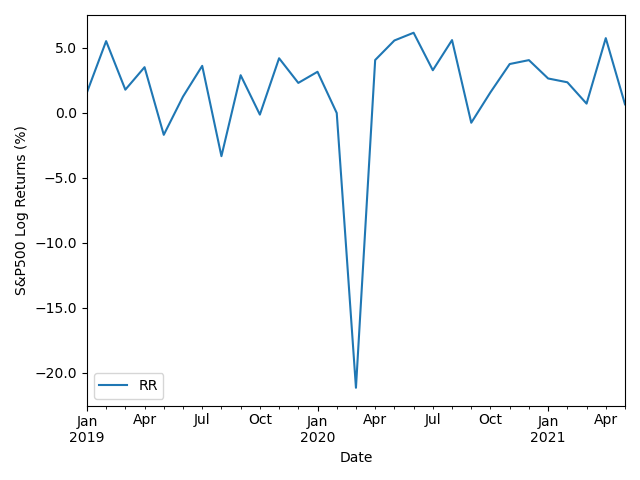
\includegraphics[width=7cm]{Graphs/SP_Data_Plot.png}
\label{fig:Results}
\end{center}
\end{figure}
\end{frame}

\begin{frame}{Data: Options}
\begin{figure}[H]
\begin{center}
\captionsetup{width=12cm, skip=5pt}
\caption{\\ \textbf{CBOE Data} \rule{12cm}{0.5pt}\\ \footnotesize{\textit{
Table shows relevant variables for S\&P500 options data. Graph shows time series of option closing prices from January 2019-May 2021. Four contracts are considered, at-the-money (ATM) and out-of-the-money (OTM) calls and puts.}}}
    \begin{minipage}{0.4\linewidth}
        \scalebox{0.7}{\begin{tabular}{ll}
\hline
 Variable Name     & Description              \\
\hline
 underlying\_symbol & Asset Symbol             \\
 quote\_date        & Quote Time               \\
 expiration        & Contract Expiration Date \\
 strike            & Contract Strike Price    \\
 option\_type       & Contract Type: Call/Put  \\
 open              & Option Price at Open     \\
 close             & Option Price at Close    \\
 high              & High Option Price        \\
 low               & Low Option Price         \\
 Volume            & Contract Trading Volume  \\
\hline
\end{tabular}}
    \end{minipage}
    \begin{minipage}{0.55\linewidth}
        \begin{center}
            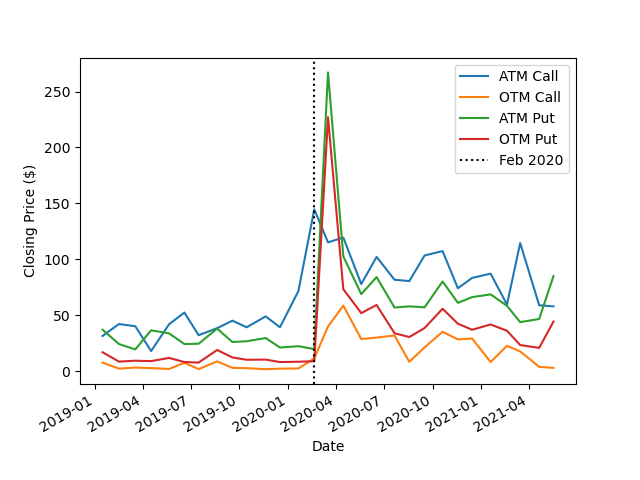
\includegraphics[width=7cm]{Graphs/Opt_Series.png}
        \end{center}
    \end{minipage}
\label{fig:Results}
\end{center}
\end{figure}
\end{frame}

\begin{frame}{Data: Risk-Free Asset}
\begin{figure}[H]
\captionsetup{width=10cm, skip=0pt}
    \begin{center}
        \caption{\\ \textbf{Risk Free Asset Returns} \rule{10cm}{0.5pt}\\ \footnotesize{\textit{Time Series of 1-Month Treasury Bill Returns from St. Louis FRED. Time span is from August 2001 to August 2021. Time span of available CBOE option data is shown in red.}}}
        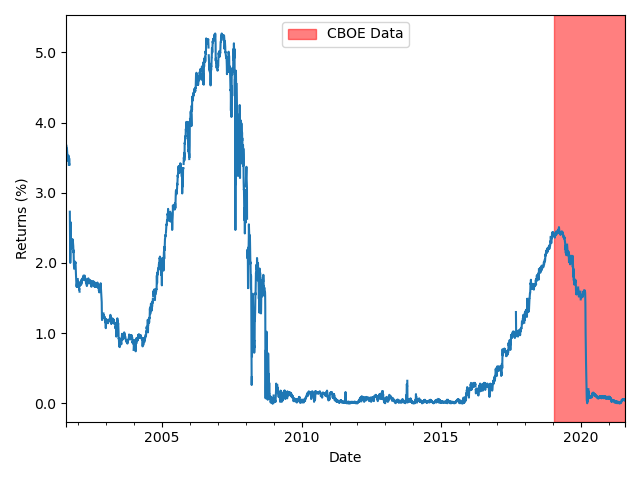
\includegraphics[width=8cm]{Graphs/Tbill_TS.png}
        \label{fig:Tbill_TS}
    \end{center}
\end{figure}
\end{frame}

\begin{frame}{Methodology}
Log returns are defined as the first difference of the log of the average monthly S\&P500 closing price:

\[y_{t} = log(S_{t}) - log(S_{t - 1})\]

Standardized returns based on fitted volatility, defined later, are $\hat{\epsilon}_{t} = \frac{y_{t}}{\hat{\sigma_{t}}}$. Simulated log returns are generated using a bootstrapped distribution of historic $\hat{\epsilon}_{t}$.

\[\textcolor{Cobalt}{y^{n}_{t + h}} = \hat{\sigma}_{t + h} \textcolor{Cobalt}{\epsilon^{n}_{t + h}} \quad \forall n \in N \ and \ \forall h \in T - t\]

\vspace{1cm}

Simulated option returns are calculated from simluated prices $\textcolor{Cobalt}{S_{t + h|t+h-1}^{n}} = S_{t + h - 1} e^{\textcolor{Cobalt}{y_{t + h}^{n}}}$.
\noindent
\begin{align} 
\nonumber \textcolor{Cobalt}{C_{t+1 \mid t}^{n}(k)} &= \max (\textcolor{Cobalt}{S_{t+1 \mid t}^{n}} - k, 0) \quad \quad k = K_{t, c_{1}}, \cdots, K_{t, c_{C}} 
\\ \nonumber \textcolor{Cobalt}{P_{t+1 \mid t}^{n}(k)} &= \max (k - \textcolor{Cobalt}{S_{t+1 \mid t}^{n}}, 0) \quad \quad k = K_{t, p_{1}}, \cdots, K_{t, p_{P}}
\\ \nonumber \textcolor{Cobalt}{r_{t+1 \mid t, c}^{n}(k)} &= \frac{\textcolor{Cobalt}{C_{t+1 \mid t}^{n}(k)}}{C_{t, k}} - 1 \quad \quad k = K_{t, c_{1}}, \cdots, K_{t, c_{C}}
\\ \nonumber \textcolor{Cobalt}{r_{t+1 \mid t, p}^{n}(k)} &= \frac{\textcolor{Cobalt}{P_{t+1 \mid t}^{n}(k)}}{P_{t, k}} - 1 \quad \quad k = K_{t, p_{1}}, \cdots, K_{t, p_{P}}
\end{align}
\end{frame}

\begin{frame}{Methodology}
Formally, in this paper I optimize the simulated wealth of the next period $
\textcolor{Cobalt}{A_{t + 1 \mid t}^{n}}$. This is an empirical approximation of the conditional expected utility that has LLN convergence. The optimization is therefore:
\[\max_{\mathbf{W}_{t}} \frac{1}{N} \sum_{n = 1}^{N} U(\textcolor{Cobalt}{A_{t+1 \mid t}^{n}})\]
Where $\mathbf{W}_{t}$ is the vector of allocated weights, n is a single simulation, and N is the number of simulations. This returns a vector of optimized weights $\mathbf{W}_{t}^{*}$.

\vspace{1cm}
The utility function U is:
\[U(A)=\left\{\begin{array}{ll}\frac{1}{1-\gamma} A^{1-\gamma}, & \text { if } \gamma \neq 1 \\ \log (A), & \text { if } \gamma=1\end{array}\right.\]
where $\gamma$ is the CRRA risk aversion parameter. $\gamma$ is set to 10, higher than 4 found in \cite{bliss2004option}, to induce shrinkage in the weights on the risky asset.
\end{frame}

\begin{frame}{Methodology}
I assume that the log returns follow a normal distribution with a time varying volatility term, which is modeled by a GARCH(1, 1) process. Formally:

\begin{align}
\nonumber y_{t} &= \sigma_{t} \epsilon_{t} \quad \epsilon_{t} \sim iid.N(0, 1)
\\ \nonumber \sigma_{t}^{2} &= \omega + \alpha y_{t - 1}^{2} + \beta \sigma_{t - 1}^{2}
\\ \nonumber & \omega > 0 \ \ \alpha, \beta \geq 0
\end{align}
\end{frame}

\begin{frame}{Methodology}
Simulated next period wealth is formulated as current wealth times the simulated total return of the basket of options, dependent on the choice variable $\mathbf{W}_{t}$

\[\textcolor{Cobalt}{A_{t+1 \mid t}^{n}} = A_{t}(1 + \textcolor{Cobalt}{rp_{t + 1 \mid t}^{n}}(\mathbf{W}_{t}))\]

Where $\textcolor{Cobalt}{rp_{t + 1 \mid t}^{n}}$ is:

\[\textcolor{Cobalt}{rp_{t + 1 \mid t}^{n}}(\mathbf{W}_{t}) = rf_{t} + \langle\mathbf{W}_{t}, \textcolor{Cobalt}{\mathbf{R}_{t+1 \mid t}^{n}}\rangle\]
With:
\[\textcolor{Cobalt}{\mathbf{R}_{t+1|t}^{n}} = \begin{bmatrix} \textcolor{Cobalt}{r_{t + 1|t, c_{1}}^{n}}, \dotsb, \textcolor{Cobalt}{r_{t + 1|t, c_{C}}^{n}}, \textcolor{Cobalt}{r_{t + 1|t, p_{1}}^{n}}, \dotsb, \textcolor{Cobalt}{r_{t + 1|t, p_{P}}^{n}} \end{bmatrix} - \begin{bmatrix} rf_{t}, \dotsb, rf_{t} \end{bmatrix}\]

\vspace{1cm}
This quantity is used to optimize $\mathbf{W}_{t}$, which is independent of current wealth $A_{t}$.
\end{frame}

\begin{frame}{Results}
\begin{figure}[H]
\begin{center}
\captionsetup{width=12cm, skip=5pt}
\caption{\\ \textbf{ExPost Results vs. S\&P500} \rule{12cm}{0.5pt}\\ \footnotesize{\textit{Summary of returns, portfolio optimization vs. S\&P500, along with graph of cumulative returns including risk-free asset. Mean, Std, Min, and Max are percentages. Period spans from January 2019 to May 2021.}}}
    \begin{minipage}{0.53\linewidth}
        \centerline{\begin{tabular}{lrrrrrrr}
\hline
         &   Mean &   Std &   Min &   Max &   Skew &   Kurtosis &   SR \\
\hline
 S\&P 500 &    1.8 &   4.7 & -19.1 &   6.3 &  -3.14 &      11.59 & 0.38 \\
 ExPost  &    0.7 &   5.0 & -19.9 &  11.5 &  -2.22 &       9.15 & 0.15 \\
\hline
\end{tabular}}
    \end{minipage}
    \begin{minipage}{0.8\linewidth}
        \begin{center}
            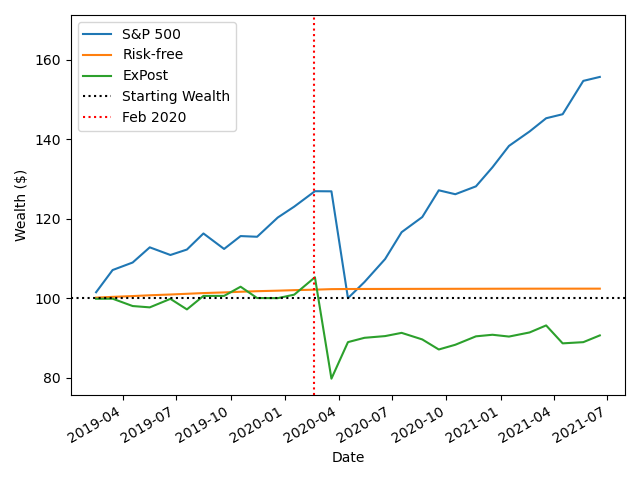
\includegraphics[width=7cm]{Graphs/Cum_Returns.png}
        \end{center}
    \end{minipage}
\label{fig:Results}
\end{center}
\end{figure}
\end{frame}

\begin{frame}{Results}
\begin{figure}[H]
\captionsetup{width=11cm, skip=0pt}
    \begin{center}
        \caption{\\ \textbf{Portfolio Optimization Weights by Contract} \rule{11cm}{0.5pt}\\ \footnotesize{\textit{Optimized weights from portfolio optimization are shown by option type, as well as for the call-put difference and risk-free assset. The time period is January 2019 to May 2021.}}}
        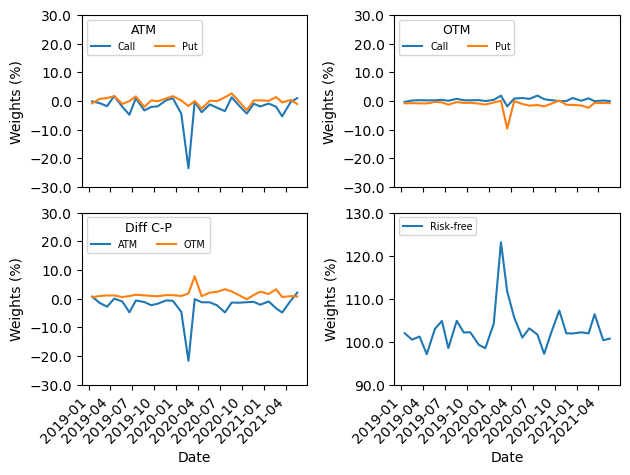
\includegraphics[width=7cm]{Graphs/WeightsPlot.png}
        \label{fig:Weights}
    \end{center}
\end{figure}
\end{frame}

\begin{frame}{Conclusion}
    \begin{itemize}
        \item Portfolio optimization returns show a sharpe ratio of -0.04 vs. 0.33 for the underlying S\&P500 in the time period.
        \item The ex-post returns do, however, show a lower skew and kurtosis, meaning the returns are closer to normality, even with the Covid months.
        \item Removing February and March of 2020 results in a sharpe ratio of 0.14. These months represent 6\% of the sample, so a larger sample with less weight on these months may impact results. Doing the same for the S\&P500 results in a Sharpe Ratio of 1.02.
    \end{itemize}
\end{frame}

\begin{frame}{Future Work}
    \begin{itemize}
        \item Options can only be traded in integer quantities. Imposing this constraint on the weights would result in a non-convex feasible set, increasing both computational complexity and real world applicability of the solution.
        \item Combing the simulation approach of \cite{faias2017optimal} and the dynamic rebalancing of \cite{zhao2018markowitz} could result in a more profitable model, but additional model specification.
        \item Incorporating a larger set of contracts (multiple underlying assets, maturities, futher OTM) could yield better results through a larger choice set, but also expose model to low liquidity risks and contract redundancy.
        \item Other models for simluating future returns may prove to be more effective than GARCH in this setting, including ones that better incorporate real time information such as sentiment analysis models.
    \end{itemize}
\end{frame}

\begin{frame}
\begin{center}
\large{Thank you for listening!}
\end{center}
\end{frame}

\begin{frame}{References}
% \nocite{*}
\bibliography{References}    
\end{frame}


\begin{frame}{Notes}
    \begin{itemize}
        \item Average risk-free return from 2001-2013 is 1.57 times higher than 2019-2021.
        \item The result of a spike in weight on the risk-free asset is consistent with risk aversion in anticipation of a crisis.
        \item GARCH doesn't take into account any anticipation of future events, only price and volatility information that is available in the underlying asset.
        \item Back in February-March 2020, there was uncertainty about how governments would respond to the crisis. Both the markets and average people were unsure about the level of stimulus and money printing central banks would engage in. Based on the spike in puts at the March contract with April expiration, the options markets thought the S\&P500 would continue to decline, while in reality in bounced back, in part due to unprecendented aggressive government intervention.
        \item This is a downside of the hold until expiration strategy, future losses were baked in after the trade was made. A dynamic rebalancing strategy could have theoretically shed the unprofitable positions earlier and mitigated loss as markets adjusted to new information.
    \end{itemize}
\end{frame}

\begin{frame}{Notes}
    \begin{itemize}
        \item Eraker, F/SC, and others have found that option returns are not adequately modeled by their first and second moments, so including higher level moments through the utility function allows this non standard distribution to be more effectively accounted for.
        \item Skew, kurtosis values of standardized returns indicate GARCH may not even be an appropriate model.
        \item While the most extreme weight in this sample was actually profitable, choosing extreme weights in other settings may not be.
        \item The power utility function is able to take into account deeper moments of the returns distribution in the optimization depending on gamma.
        \item Options are duplicated into short and long options to incorporate transaction costs, short options enter the model multiplied by -1.
    \end{itemize}
\end{frame}

\end{document}